\documentclass[11pt,letterpaper]{article}

\addtolength{\oddsidemargin}{-.875in}
\addtolength{\evensidemargin}{-.875in}
\addtolength{\textwidth}{1.75in}

\addtolength{\topmargin}{-.875in}
\addtolength{\textheight}{1.75in}

\usepackage[utf8]{inputenc}
\usepackage{caption} % for table captions
\usepackage{amsmath} % for multi-line equations and piecewises
\DeclareMathOperator{\sign}{sign}
\usepackage{graphicx}
\usepackage{relsize}
\usepackage{xspace}
\usepackage{verbatim} % for block comments
\usepackage{subcaption} % for subfigures
\usepackage{enumitem} % for a) b) c) lists
\usepackage{tabularx}
\usepackage{color}
\usepackage{multirow}
\usepackage{float}
\usepackage[acronym,toc]{glossaries}

\newacronym{ANL}{ANL}{Argonne National Laboratory}
\newacronym{B4C}{B4C}{boron carbide}
\newacronym{BSD}{BSD}{Berkeley Software Distribution}
\newacronym{CR}{CR}{control rod}
\newacronym{DOE}{DOE}{Department of Energy}
\newacronym{EOEC}{EOEC}{end of equilibrium cycle}
\newacronym{FDM}{FDM}{Finite Difference Method}
\newacronym{FEM}{FEM}{Finite Element Method}
\newacronym{FSV}{FSV}{Fort St. Vrain}
\newacronym{GRS}{GRS}{Gesellschaft für Anlagen und Reaktorsicherheit}
\newacronym{He}{He}{helium}
\newacronym{HZDR}{HZDR}{Helmholtz-Zentrum Dresden-Rossendorf}
\newacronym{HTGR}{HTGR}{High Temperature Gas-Cooled Reactor}
\newacronym{HTR}{HTR}{High Temperature Reactor}
\newacronym{HTTR}{HTTR}{High Temperature Test Reactor}
\newacronym{IPyC}{IPyC}{inner pyrolitic carbon}
\newacronym{INL}{INL}{Idaho National Laboratory}
\newacronym{KAERI}{KAERI}{Korea Atomic Energy Research Institute}
\newacronym{LBP}{LBP}{Lumped Burnable Poison}
\newacronym{LGPL}{LGPL}{Lesser GNU Public License}
\newacronym{LWR}{LWR}{Light Water Reactor}
\newacronym{MC}{MC}{Monte Carlo}
\newacronym{MHTGR}{MHTGR}{Modular High-Temperature Gas-Cooled Reactor}
\newacronym{MOOSE}{MOOSE}{Multiphysics Object-Oriented Simulation Environment}
\newacronym{MSR}{MSR}{Molten Salt Reactor}
\newacronym{NEA}{NEA}{Nuclear Energy Agency}
\newacronym{NEM}{NEM}{Nodal Expansion Method}
\newacronym{NGNP}{NGNP}{Next Generation Nuclear Power}
\newacronym{NRC}{NRC}{Nuclear Regulatory Commission}
\newacronym{NSC}{NSC}{Nuclear Science Committee}
\newacronym{OECD}{OECD}{Organisation for Economic Co-operation and Development}
\newacronym{OPyC}{OPyC}{outer pyrolitic carbon}
\newacronym{ORNL}{ORNL}{Oak Ridge National Laboratory}
\newacronym{OS}{OS}{Operator-Splitting}
\newacronym{PBMR}{PBMR}{Pebble Bed Modular Reactor}
\newacronym{PDE}{PDE}{Partial Differential Equation}
\newacronym{PMR}{PMR}{Prismatic Modular Reactor}
\newacronym{RSC}{RSC}{Reserve Shutdown Control}
\newacronym{RSD}{RSD}{Relative Standard Deviation}
\newacronym{SD}{SD}{Standard Deviation}
\newacronym{SiC}{SiC}{silicon carbide}
\newacronym{SNU}{SNU}{Seoul National University}
\newacronym{TIP}{TIP}{transverse integration procedure}
\newacronym{TRISO}{TRISO}{Tristructural Isotropic}
\newacronym{UIUC}{UIUC}{University of Illinois at Urbana-Champaign}
\newacronym{UNIST}{UNIST}{Ulsan National Intitute of Science and Technology}
\newacronym{UK}{UK}{United Kingdom}
\newacronym{UMICH}{UMICH}{Universtiy of Michigan}
\newacronym{US}{US}{United States}
\newacronym{VHTR}{VHTR}{Very High Temperature Gas Cooled Reactor}
%\newacronym{<++>}{<++>}{<++>}
%\newacronym{<++>}{<++>}{<++>}

\definecolor{bg}{rgb}{0.95,0.95,0.95}
\newcolumntype{b}{X}
\newcolumntype{f}{>{\hsize=.15\hsize}X}
\newcolumntype{s}{>{\hsize=.5\hsize}X}
\newcolumntype{m}{>{\hsize=.75\hsize}X}
\newcolumntype{r}{>{\hsize=1.1\hsize}X}
\usepackage{titling}
\usepackage[hang,flushmargin]{footmisc}
\renewcommand*\footnoterule{}
\usepackage{tikz}
\usepackage{array}
\usepackage{booktabs,mathptmx,siunitx}
\sisetup{input-symbols = {()},  % do not treat "(" and ")" in any special way
         group-digits  = false} % no grouping of digits

\usetikzlibrary{shapes.geometric,arrows}
\tikzstyle{process} = [rectangle, rounded corners,
minimum width=1cm, minimum height=1cm,text centered, draw=black,
fill=blue!30]
\tikzstyle{arrow} = [thick,->,>=stealth]

\graphicspath{}

\begin{document}

\section{Introduction}

The main objective of this study is to determine if a space reactor can achieve a core lifetime of 10 years.

\section{Reactor model}

Table \ref{tab:design} displays the main design parameters of the reactor.
We modeled two reactor designs: (1) a bare reactor, and (2) a reactor with reflectors in all its sides.
With the main design parameters, we calculated the reactor sizes.
We imposed the active core height to be equal to the active core diameter.

\begin{table}[htbp!]
	\centering
	\caption{Reactor main design parameters.}
	\label{tab:design}
	\begin{tabular}{@{}l c}
	\toprule
	Characteristic 		& Value			\\
	\midrule
	Shape 				& Cylindrical 	\\
	Total weight 		& 3000 kg		\\
	Power		 		& 100 kW		\\
	Fuel form			& TRISO particle 	\\
	Fuel material		& UCO ($\varepsilon$ = 20\%)	\\
	Packing fraction 	& 42\%			\\
	Matrix				& Zr-hydride	\\
	\bottomrule
	\end{tabular}
\end{table}

Table \ref{tab:design} shows the main characteristics of both models.
The moderator material is Zr-hydride (ZrH).
ZrH has 3 different phases: $\gamma$-ZrH, $\delta$-ZrH$_{1.5}$, and $\varepsilon$-ZrH$_{2}$.
We chose phase $\delta$-ZrH$_{1.5}$ for this work.
For the reflector material, we chose Beryllium (Be) in metal form.
Table \ref{tab:densities} exhibits the density of the materials.

\begin{table}[htbp!]
	\centering
	\caption{Reactor main characteristics.}
	\label{tab:design}
	\begin{tabular}{@{}l c}
	\toprule
	Shared characteristics		& Value	\\
	\midrule
	UCO radius	        		& 0.02125 cm \cite{oecd_nea_benchmark_2017} \\
	Buffer radius       		& 0.03125 cm \cite{oecd_nea_benchmark_2017} \\
	IPyC radius         		& 0.03475 cm \cite{oecd_nea_benchmark_2017} \\
	SiC radius          		& 0.03825 cm \cite{oecd_nea_benchmark_2017} \\
	OPyC radius         		& 0.04225 cm \cite{oecd_nea_benchmark_2017} \\
	\midrule
	Bare reactor characteristics & \\
	\midrule
	Reactor radius 				& 47.2 cm 	\\
	Reactor height 				& 94.4 cm 	\\ 
	\midrule
	Reflected reactor characteristics & \\
	\midrule
	Active core radius 			& 42 cm 	\\
	Active core height 			& 84 cm 	\\
	Top reflector thickness 	& 10 cm 	\\
	Bottom reflector thickness 	& 10 cm 	\\
	Radial reflector thickness 	& 13 cm 	\\
	\bottomrule
	\end{tabular}
\end{table}

\begin{table}[htbp!]
	\centering
	\caption{Material densities.}
	\label{tab:densities}
	\begin{tabular}{@{}l c c}
	\toprule
	Material   		& Density [g/cm$^3$] & References 	\\
	\midrule
	UCO				& 10.5	& \cite{oecd_nea_benchmark_2017} 	\\
	Buffer			& 1.0	& \cite{oecd_nea_benchmark_2017} 	\\
	PyC				& 1.9	& \cite{oecd_nea_benchmark_2017} 	\\
	SiC				& 3.2	& \cite{oecd_nea_benchmark_2017} 	\\
	ZrH				& 5.624	& \cite{weck_mechanical_2015} 	\\
	Be				& 1.8	& \cite{beeston_beryllium_1970}	\\
	\bottomrule
	\end{tabular}
\end{table}

The choice of burnup calculator was Serpent2 \cite{leppanen_development_2007} \cite{leppanen_serpent_2015}.
Figure \ref{fig:designs} shows the reactor designs geometries in Serpent2.
All the simulations considered a reactor temperature of 900 K.
The simulations ran 240 active neutron cycles with 200,000 neutrons per cycle.

\begin{figure}[htbp!]
	\centering
	\begin{subfigure}[t]{0.4\textwidth}
		\centering
		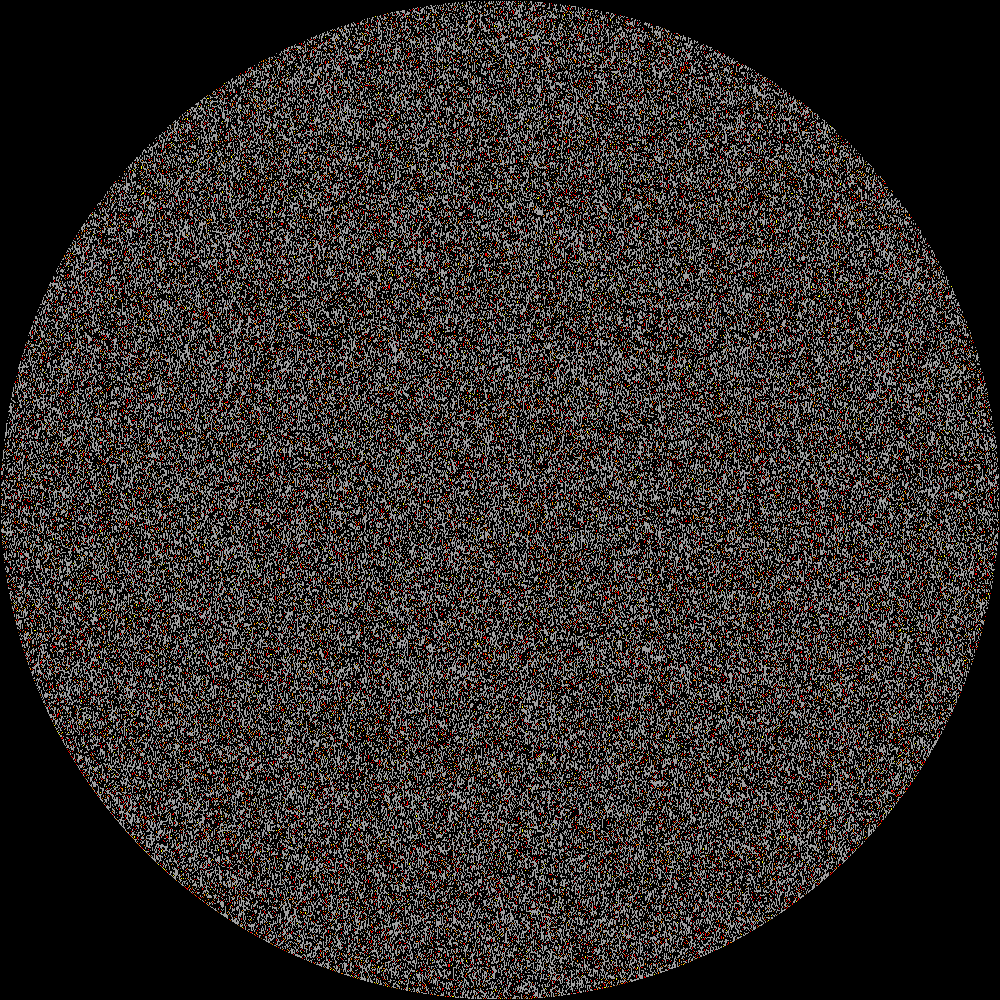
\includegraphics[width=\linewidth]{figures/bare2_geom1.png}
		\caption{Bare reactor.}
	\end{subfigure}
	\begin{subfigure}[t]{0.4\textwidth}
		\centering
		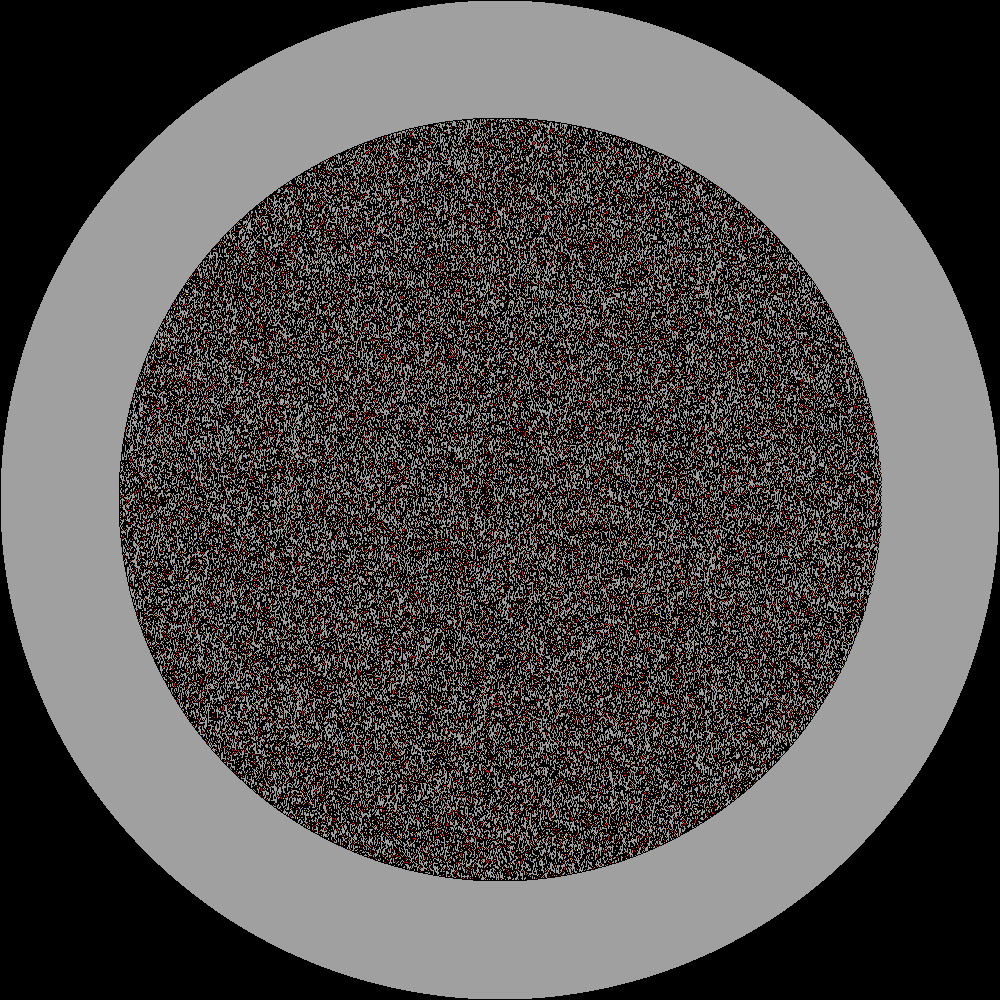
\includegraphics[width=\linewidth]{figures/reflector2_geom1.png}
		\caption{Reflected reactor.}
	\end{subfigure}
	\hfill
	\caption{Serpent model of the different designs.}
	\label{fig:designs}
\end{figure}

\section{Results}

Figure \ref{fig:results-bare2} and \ref{fig:results-reflector2} display the results for the different reactor models.
Both designs have a core lifetime of at least 10 years.
The addition of the reflector to the model increases the reactor lifetime and decreases the initial mass of U-235 by around a 30\%.

\begin{figure}[htbp!]
	\centering
	\begin{subfigure}[t]{0.4\textwidth}
		\centering
		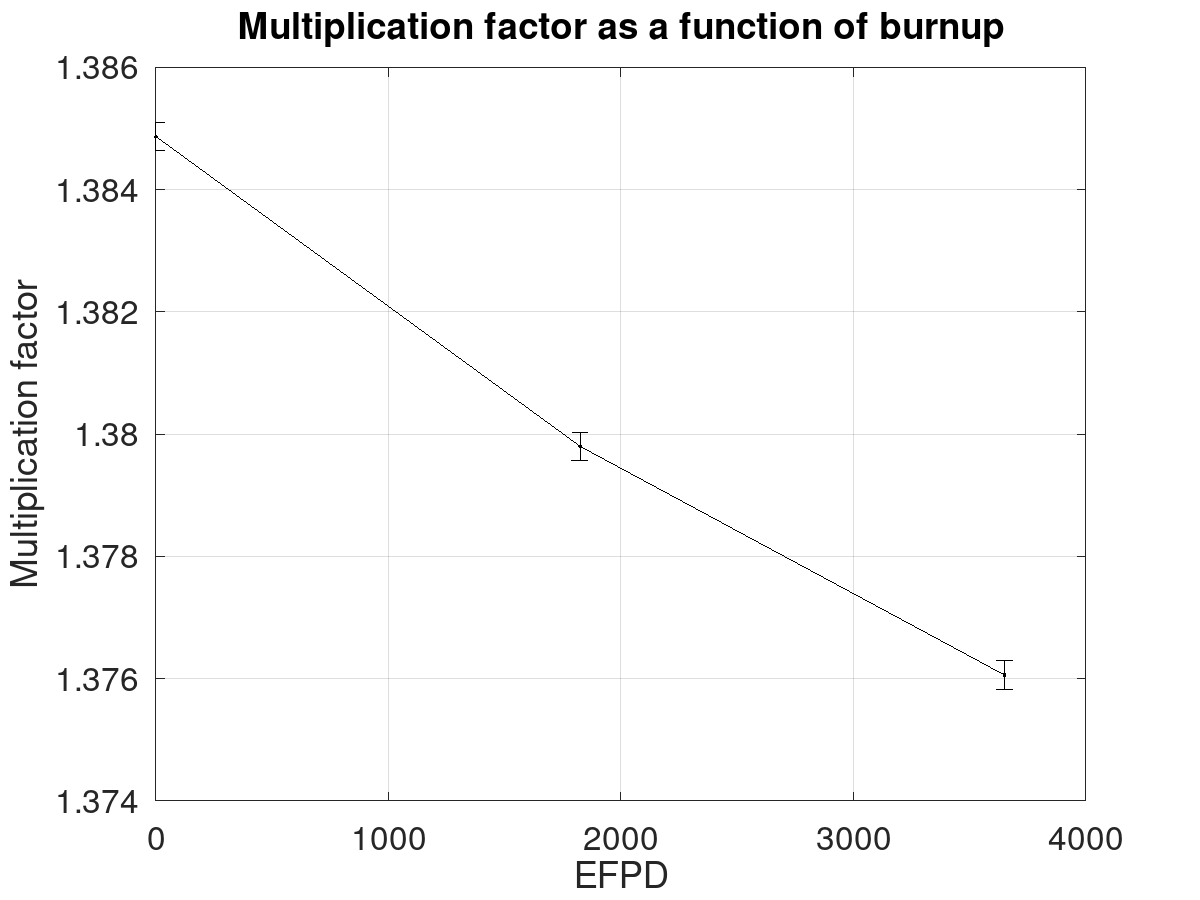
\includegraphics[width=\linewidth]{figures/bare2-Keff.png}
		\caption{$K_{eff}$ as a function of burnup.}
	\end{subfigure}
	\begin{subfigure}[t]{0.4\textwidth}
		\centering
		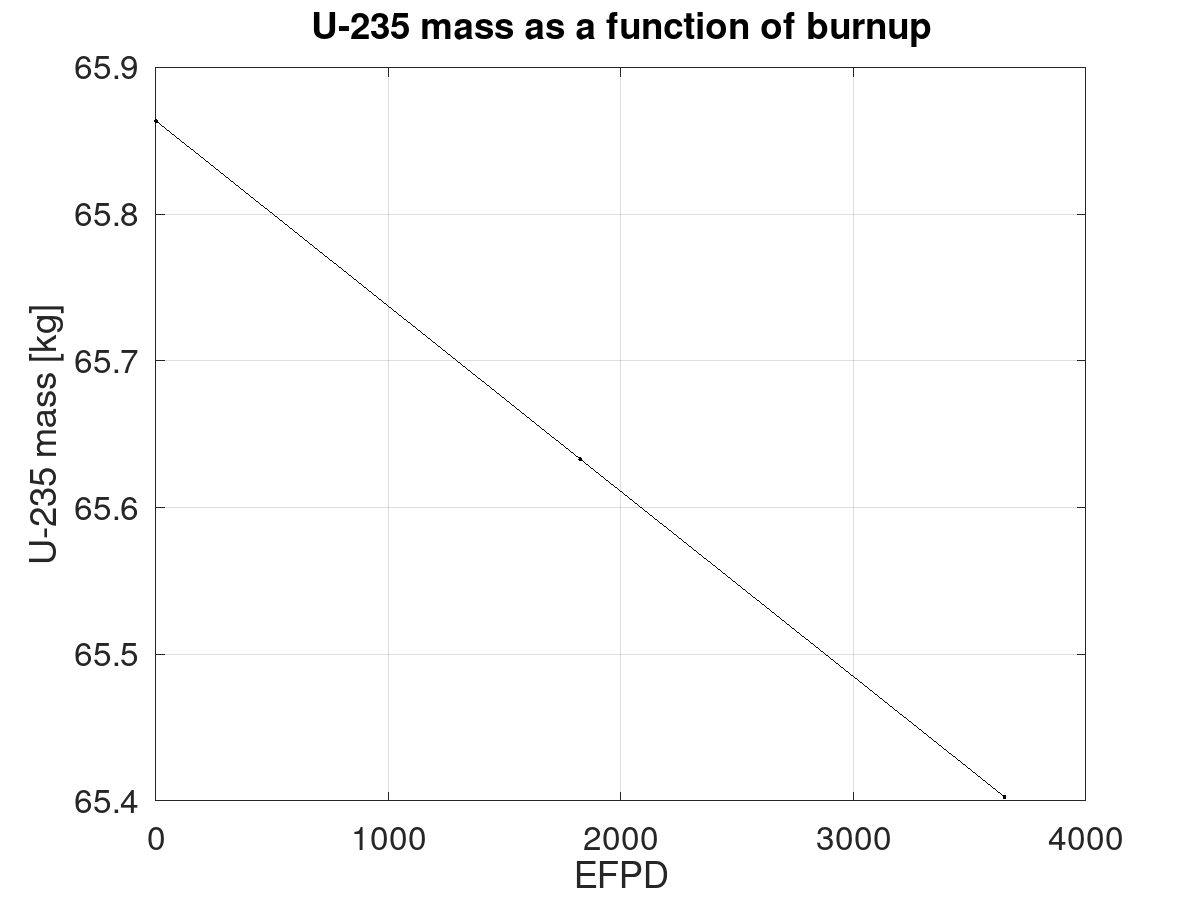
\includegraphics[width=\linewidth]{figures/bare2-mU235.png}
		\caption{U-235 mass as a function of burnup.}
	\end{subfigure}
	\hfill
	\caption{Bare reactor parameter change over burnup.}
	\label{fig:results-bare2}
\end{figure}

\begin{figure}[htbp!]
	\centering
	\begin{subfigure}[t]{0.4\textwidth}
		\centering
		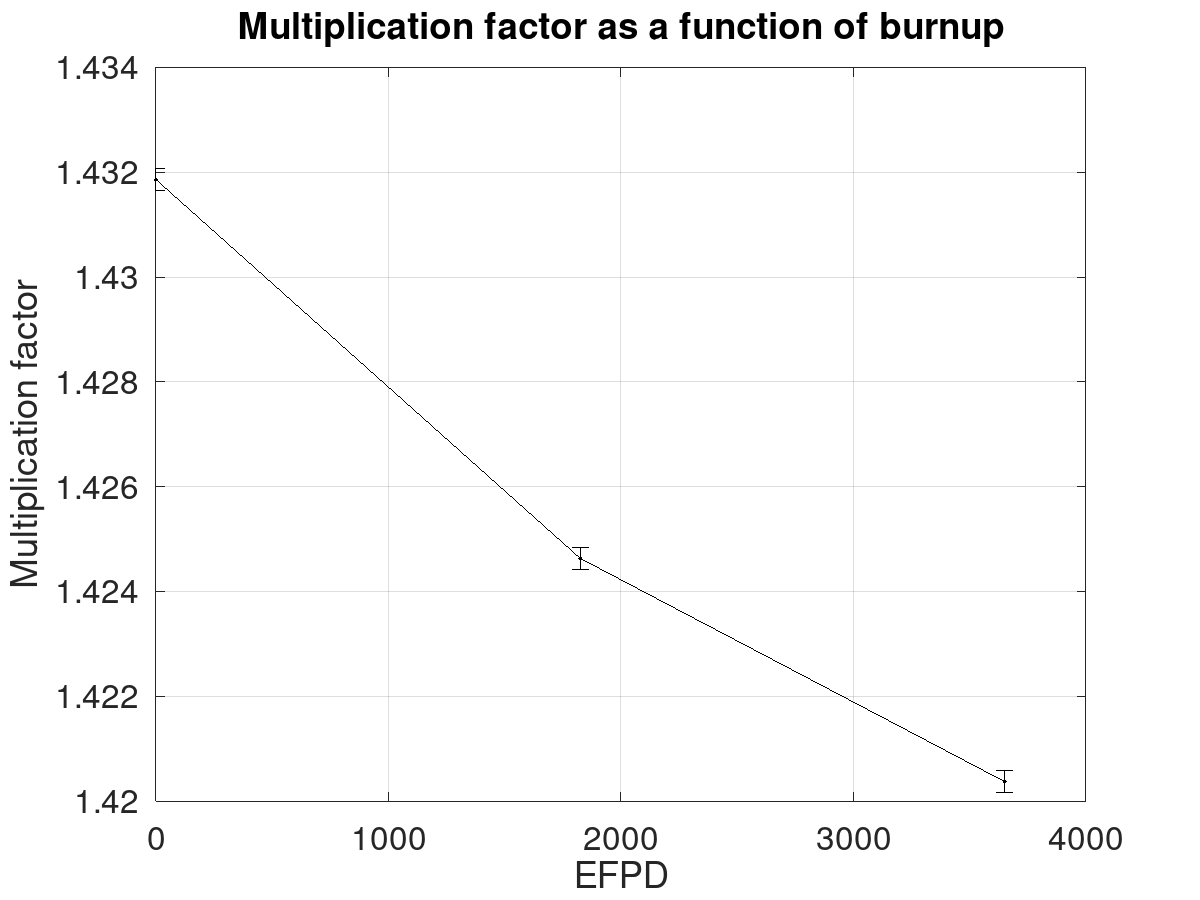
\includegraphics[width=\linewidth]{figures/reflector2-Keff.png}
		\caption{$K_{eff}$ as a function of burnup.}
	\end{subfigure}
	\begin{subfigure}[t]{0.4\textwidth}
		\centering
		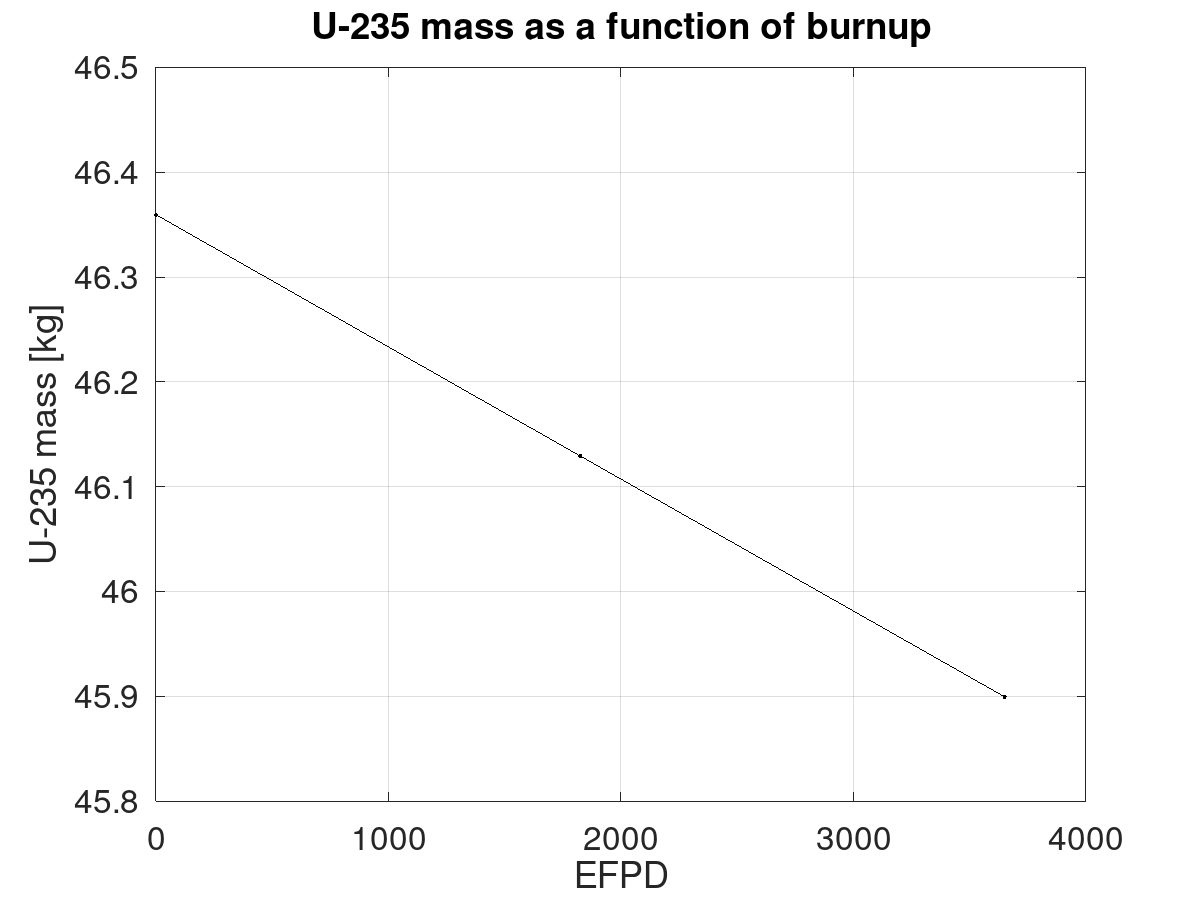
\includegraphics[width=\linewidth]{figures/reflector2-mU235.png}
		\caption{U-235 mass as a function of burnup.}
	\end{subfigure}
	\hfill
	\caption{Reflected reactor parameter change over burnup.}
	\label{fig:results-reflector2}
\end{figure}

\pagebreak
\bibliographystyle{plain}
\bibliography{bibliography}

\end{document}

% \begin{figure}[htbp!]
% 	\centering
% 	\begin{subfigure}[t]{0.4\textwidth}
% 		\centering
% 		\includegraphics[width=\linewidth]{figures/radial-layout.png}
% 		\caption{XY-plane.}
% 	\end{subfigure}
% 	\begin{subfigure}[t]{0.4\textwidth}
% 		\centering
% 		\includegraphics[width=\linewidth]{figures/axial-layout.png}
% 		\caption{YZ-plane.}
% 	\end{subfigure}
% 	\hfill
% 	\caption{MHTGR reactor layout.}
% 	\label{fig:layout}
% \end{figure}

% \begin{figure}[htbp!]
% 	\centering
% 	\includegraphics[width=0.6\linewidth]{figures/axial1.png}
% 	\hfill
% 	\caption{Neutron flux on the specified fuel channel.}
% 	\label{fig:axial}
% \end{figure}

% \begin{table}[htbp!]
% \centering
% 			\caption{MHTGR350 fuel element characteristics \cite{oecd_nea_benchmark_2017}.}
% 			\label{tab:element-characteristics}
% 		\begin{tabular}{@{}l S[table-format=2.2] c}
% 		\toprule
% 		\multicolumn{1}{c}{Shared characteristics} & \multicolumn{1}{c@{}}{Value} & \multicolumn{1}{c@{}}{Units} \\
% 		\midrule
% 	Block pitch (flat-to-flat)       & 36 		 & cm       \\
% 	Fuel length                      & 79.3 	 & cm       \\
% 	Fuel handling diameter           & 3.5 		 & cm       \\
% 	Fuel handling length             & 26.4 	 & cm       \\
% 	RSC hole diameter                & 9.525 	 & cm       \\
% 	RSC center to assembly center    & 9.756 	 & cm       \\
% 	Fuel/coolant pitch               & 1.879 	 & cm       \\
% 	Fuel hole radius                 & 0.635 	 & cm       \\
% 	Compacts per fuel hole           & \multicolumn{1}{c@{}}{15}   	& -        \\
% 	Large coolant hole radius        & 0.794 	 & cm       \\
% 	Small coolant hole radius        & 0.635 	 & cm       \\
%   LBP hole radius                  & 0.635 	 & cm       \\
% 	Block graphite density           & 1.85    & g/cm$^3$ \\
% 	\midrule

% 			\multicolumn{1}{c}{Standard element} &  &  \\

% 	\midrule
% 	Number of large coolant holes    & \multicolumn{1}{c@{}}{120}   & -        \\
% 	Number of small coolant holes    & \multicolumn{1}{c@{}}{6}   	& -        \\
% 	Number of fuel holes             & \multicolumn{1}{c@{}}{210}  	& -        \\
% 	\midrule

% 			\multicolumn{1}{c}{RSC element} &  &  \\

% 	\midrule
% 	Number of large coolant holes    & \multicolumn{1}{c@{}}{88}    & -        \\
% 	Number of small coolant holes    & \multicolumn{1}{c@{}}{7}   	& -        \\
% 	Number of fuel holes             & \multicolumn{1}{c@{}}{186}  	& -        \\
% 		\bottomrule
% 		\end{tabular}
% \end{table}